\chapter{Berechnung der Tonsysteme}

\begin{enumerate}[a)]
\item
Siehe MATLAB-Code:
\begin{itemize}
\item
EqualTemperamentScale.m 
\item
PythagoreanScale.m
\end{itemize}
\item
Um die gleichstufige und die pythagoräische Skala zu konstruieren, haben wir folgende Berechnungsvorschriften verwendet:

\underline{Gleichstufig:}
\\
\begin{align*}
    f(n) &= a_n \cdot f_0 \\ 
    a_n &= \sqrt[12]{2}^n \\
    n &= 0, \,... \, ,127
\end{align*} 
\underline{Pythagoräisch:}
\\
\\
Zunächst werden 12 Faktoren berechnet, die den Multiplikatoren für die Referenzfrequenz entsprechen um die erste Oktave zu erhalten.
Die Faktoren ergeben sich aus Aufeinanderschichtung reiner Quinten und anschließender gegebenfalls mehrfacher Oktavierung nach unten.
\\
Von C bis Fis wandert man im Uhrzeigersinn den Quintenzirkel entlang:

\begin{align*}
    a_n &= \frac{1.5^n}{2^m} \\
    n &= 0,  \,... \, ,6
\end{align*} 
$m$ gibt an wie oft man durch 2 teilen muss um die durch Quintschichtung erhaltenen Frequenz auf die erste Oktave zurückzuführen, d.h. ein $a_n$ zwischen 1 und 2 zu erhalten.
\\

Für die restlichen 5 Faktoren, wandert man entgegen dem Uhrzeigersinn den Quintenzirkel entlang, erniedrigt jeweils um eine reine Quinte und oktaviert gegegebenfalls mehrfach, diesmal nach oben.

\begin{align*}
    a_n &= 1.5^{-(n-6)} \cdot 2^m \\
    n &= 7, \, ... \, ,11 
\end{align*}

Die Faktoren $a_n$ werden nun in aufsteigender Reihenfolge sortiert. Die Frequenzen können dann folgendermaßen berechnet werden :

\[
    f_n = 
\begin{cases}
    a_n \cdot f_0,& \text{if } n\leq 11 \\
    f_{n-12},&\text{if } n> 11
\end{cases}  
\]

Im Code wurde für den letzten Teil eine nicht-rekursive Berechnung verwendet, um effizient zu bleiben.

\item

In Tabelle \ref{tab:t1} sind die ersten 12 berechneten Frequenzen oberhalb unseres gewählten Referenztons C$_{2}$ bzw. 16.352 Hz für die zwei Stimmungen aufgelistet. Zudem sind die Frequenzverhältnisse zum Grundton innerhalb dieser Oktave zu sehen, welche den Faktoren $a_n$ aus 1b) entsprechen. Diese Verhältnisse lassen sich in das additive Maß \glqq Musikalische Cent \grqq umrechnen, welches auf die gleichstufige Stimmung geeicht ist, in der ein Halbton genau 100 Cent entspricht. Die Formel zur Berechung bei gegebenem Frequenzverhältnis $p$ eines Intervalls $i$ lautet:

\begin{align*}
    i = 1200 \cdot \frac{\mathrm{log}(p)}{\mathrm{log} 2} \mathrm{Cent}
\end{align*}




\begin{table}
\centering
\begin{tabular}{| c | c | c | c | c | c | c | c |}
  \hline			
  Note & Intervall& Frequenz & Frequenz & Verhältnis & Verhältnis & Cent& Cent \\
  & &gleichst. & pyth. & gleichst. & pyth. & gleichst. & pyth. \\
  \hline
  C (C$_{2}$) & Prime&16.352 & 16.352 & 1.000 & 1.0000 & 0 & 0 \\
  Des/Cis & kl. Sekunde& 17.324 & 17.226 & 1.0595 & 1.0535 & 100 & 90\\
  D &gr. Sekunde &18.354 & 18.396 & 1.1225 & 1.1250 & 200 & 204\\
  Es/Dis & kl. Terz & 19.445 & 19.380 & 1.1892 & 1.1852 & 300 & 294 \\
  E & gr. Terz &20.602 & 20.695 & 1.2599 & 1.2656 & 400 & 408\\
  F & Quarte &21.827 & 21.802 & 1.3348 & 1.3333 & 500 & 498\\
  Ges/Fis & Tritonus&23.125 & 23.282 & 1.4142 & 1.4238 & 600 & 611 \\
  G & Quinte & 24.500 & 24.527 & 1.4983 & 1.5000 & 700 &  702 \\
  As/Gis & kl. Sexte& 25.957 & 25.840 & 1.5874 & 1.5802 & 800 & 792\\
  A & gr. Sexte&27.500 & 27.593 & 1.6818 & 1.6875 &  900 & 906\\
  B/Ais & kl. Septime& 29.135 & 29.070 & 1.7818 & 1.7778 & 1000 & 996 \\
  H & gr. Septime&30.868 & 31.043 & 1.8877 & 1.8984 & 1100 & 1110\\
  C (C$_{1}$)& Oktave & 32.703 & 32.703 &2.0000 &2.0000 & 1200 & 1200\\
  \hline  
\end{tabular}
\caption{Unterschiede zwischen gleichstufiger und pythagoräischer Stimmung im Bereich einer Oktave oberhalb des Referenzwerts C$_{2}$, welcher 16.352 Hz in der gleichstufigen Stimmung entspricht.}
\label{tab:t1}
\end{table}


\begin{figure}
  \centering
      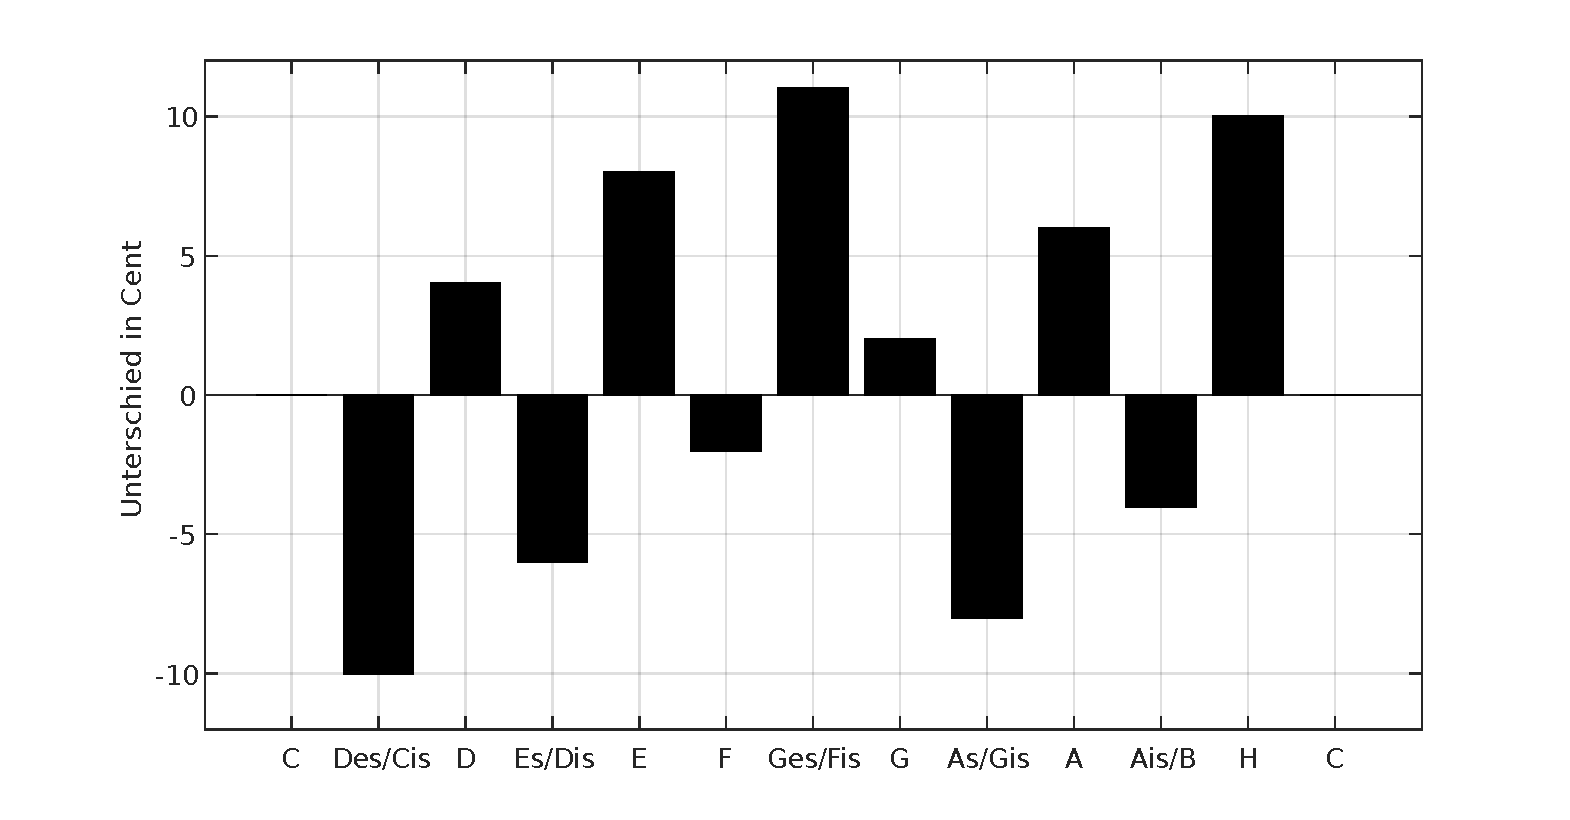
\includegraphics[width=\textwidth]{Figures/diff}
 \caption{Unterschiede zwischen gleichstufigen und pythagoräischen auf C bezogenen Intervalltönen in Cent}
	\label{fig:f1}
\end{figure}







\end{enumerate}